\documentclass[a4paper,12pt]{article}

\renewcommand{\labelenumii}{\theenumii}
\renewcommand{\theenumii}{\theenumi.\arabic{enumii}.}

\usepackage[T2A]{fontenc}
\usepackage[utf8]{inputenc}
\usepackage[english,russian]{babel}
\usepackage{hyperref}
\usepackage{graphicx}
\graphicspath{{lab2_images/}}
\usepackage[a4paper, total={8in, 10in}]{geometry}

\begin{document}
	\begin{enumerate}
		\item \begin{enumerate}
			\item Как устроен стековый фрейм на x86\_64 для System V ABI?\\
			\textbf{Ответ:}\\
			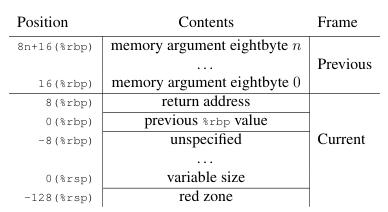
\includegraphics{stack_frame.jpg}\\
			Стэк растёт от старших адресов к младшим.
			
			\item Как передаются аргументы?\\
			\textbf{Ответ:}\\
			
			
			\item Как получить возвращаемое значение из функции?\\
			\textbf{Ответ:}\\
			
			
			\item Восстановление стек трейса, как можно реализовать в программе?\\
			\textbf{Ответ:}\\
			
			
			\item Как узнать, когда перестать раскручивать фрейм?\\
			\textbf{Ответ:}\\
			
			
			\item Что можно сделать, если код не выделяет стековый фрейм явным образом\\ (-fomit-frame-pointer)?\\
			\textbf{Ответ:}\\
			
			
		\end{enumerate}
	\item \begin{enumerate}
		\item Где аллоцируется стек ядра, стек прошивки?\\
		\textbf{Ответ:}\\
		
		
		\item Когда JOS использует тот или иной стек, когда перестаёт использовать стек прошивки?\\
		\textbf{Ответ:}\\
		
		
		\item Всегда ли стек доступен?\\
		\textbf{Ответ:}\\
		
		
		\item Почему нельзя переиспользовате стек прошивки в ядре?\\
		\textbf{Ответ:}\\
		
		
		\end{enumerate}
	\item \begin{enumerate}
		\item Как запускается JOS на 32-битной прошивке UEFI?\\
		\textbf{Ответ:}\\
		
		
		\item В чём отличия от 64-битного запуска?\\
		\textbf{Ответ:}\\
		
		
		\item Зачем нужен head64 (bootstrap.S) при запуске JOS?\\
		\textbf{Ответ:}\\
		
		
		\item Можно ли было избежать его реализации (объединив его код с entry.S)?\\
		\textbf{Ответ:}\\
		
		
		\end{enumerate}
	\end{enumerate}
"в rbp лежит адрес предыдущего значения rbp, которое указывает на следующий и так далее. 
Первый rbp = 0 устанавливается в entry.S. Очевидно, можно идти в цикле по этим значениям и восстанавливать фреймы.
Над rbp в стеке лежит адрес возврата. По этому адресу, используя отладочную информацию, можно узнать,
какая функция вызывала текущую и вывести ее имя, файл и т.д.
Если используется флаг -fomit-frame-pointer, значения rbp в стеке не сохраняются, и отладка сильно затрудняется.
Можно попробовать идти начиная с адреса возврата, прибавляя к указателю значение выравнивания стека, проверять, есть ли
перед этим адресом вызов нашей функции и если есть искать в отладочной информации адрес начала и название той функции, 
в которую происходит возврат."\\\\
"32 реальный режим -> защищенный режим\\
64 реальный режим -> защищенный режим -> длинный режим\\
В Trampline.c в 32бит в отличие от 64бит вызывается CallKernelThroughGateAsm() - переход в лонг мод. И еще куча проверок, поддерживает ли железо 64бит\\
Далее вызывается bootstrap.s (head64), entry.S (entry)\\
PS  вместо двух разных файлов можно написать большой  \#ifdef  в одном фаиле"\\\\
Стек прошивки, аллоцируется на стадии PEI после инициализации памяти. Используется он вплоть до передачи управления ядру (в файл bootstrap.S, jmpq *\%rax).  В функцию entry (entry.S) управление передается без стека, а entry инициализирует собственный стек, который выделяется в секции .data Зачем менять стек? До вызова ядра uefi имеет свою таблицу памяти. Непосредственно перед вызовом ядра вызывается ExitBootServices(), которая освобождает некоторые регионы из этой таблицы. В частности, освобождается EfiBootServicesData, в которой хранится стек. Подробнее это описано вот здесь \href[]{https://forge.ispras.ru/projects/oscourse-2020-msu/wi..}{wiki} Если мы не поменяем стек, кто-то в будущем сможет выделить эту память себе.\\\\
"Стек ядра аллоцируется в entry.s
Стек прошивки, скорее всего, аллоцируется на стадии PEI после инициализации памяти. Используется он вплоть до передачи
управления ядру (в файл bootstrap.S). Далее в функцию entry (entry.S) управление передается без стека, а entry инициализирует
собственный стек, который выделяется в секции .data при загрузке elf-файла"\\\\
Стековый фрейм функции (stack frame) – область памяти, выделяемая всякий раз, когда вызывается функция. Трассировка стека - отчет из активных кадров стека в определенный момент времени во время выполнения программы.  Системные регистры стека:      • Указатель стека, esp, предназначается для того, чтобы указывать на верхушку стека. Вплотную к верхушке всегда находится объект, который  был добавлен в стек, но еще оттуда не снят. Хранимый в регистре esp адрес изменяется по мере того, как объекты добавляются и снимаются со стека, однако он всегда указывает на последний добавленный и еще не снятый со стека объект. Многие процессорные инструкции изменяют значение регистра esp как побочный результат своего выполнения.      • Далее на очереди еще один регистр, используемый для отслеживания позиций в стеке – регистр ebp – базовый указатель или указатель базы стекового кадра. Данный регистр предназначен для того, чтобы указывать на позицию в стековом кадре. Благодаря регистру ebp текущая функция всегда имеет своего рода точку отсчёта для доступа к аргументам и локальным переменным. Хранимый в регистре адрес изменяется, когда функция начинает или прекращает выполнение. !!!последовательность стековых кадров в стеке оказывается организованной в связный список, и регистр ebp хранит ссылку на первый элемент этого списка. Вот с опорой на это и реализованы трассировка стека в отладчиках!!!                             Команда call – основная команда для существования функции. Команда позволяет выполнить другую часть кода, запомнив при этом адрес точки возврата в стеке. Для этого команда call работает следующим образом: 1) проталкивает в стек адрес следующей команды, который является адресом точки возврата – точки, куда процессор передаст управление (возвратится) после выполнения функции; 2) передает управление по указанному в команде call адресу для выполнения команд функции. А команда ret делает противоположное. Ее задача состоит в том, чтобы возвратиться из вызываемой функции к команде, следующей за командой  call. Для этого команда ret выполняет следующие действия: 1) извлекает из стека сохраненный адрес точки возврата; 2) передает управление по только что извлеченному из стека адресу точки возврата. в rbp лежит адрес предыдущего значения rbp, которое указывает на следующий и так далее. Первый rbp = 0 устанавливается в entry.S. Очевидно, можно идти в цикле по этим значениям и восстанавливать фреймы. Над rbp в стеке лежит адрес возврата. По этому адресу, используя отладочную информацию, можно узнать, какая функция вызывала текущую и вывести ее имя, файл и т.д. Если используется флаг -fomit-frame-pointer, значения rbp в стеке не сохраняются, и отладка сильно затрудняется. Можно попробовать идти начиная с адреса возврата, прибавляя к указателю значение выравнивания стека, проверять, есть ли перед этим адресом вызов нашей функции и если есть искать в отладочной информации адрес начала и название той функции, в которую происходит возврат. полезные ссылки: \href[]{https://habr.com/ru/company/smart\_soft/blog/234239/ }{habr} \href[]{https://ru.qaz.wiki/wiki/Stack\_trace  }{wiki}\\\\
"Выравнивание памяти - требование к адресам в памяти, куда сохраняются данные. В общем видел, необходимо для увеличения быстродействия, за счёт уменьшения обращений к памяти и вспомогательных операций. Пример, int64 кладём по адресу 0x01. Чтобы его достать нужно два раза сходить в память: 0x00 и 0x08, а затем ""склеить"" байтики, чтобы получить в регистре int64.  
head64 это точка входа(entry) в формате ELF, т.е. адрес, куда передаётся управления для начала исполнения кода ядра после его загрузки/подготовки. 
Нельзя объединить код head64 и entry, т.к. head64 подготавливает/устанавливает адрес структуры, описывающей paging в CR3 и работает в lower memory, а entry сидит уже в high memory. 
Про выравнивание стэка 
System V x86-64 ABI.pdf (есть на forge):
Граница стека должна быть выровнена по адресу кратному 16 (32 or 64, если \_\_m256 \_\_m512 в регистре AVX)
Зачем: для увеличения скорости доступа процессора к памяти из ОЗУ

В JOS (доп вопрос):
в файле entry.S директива 
.p2align PAGE\_SHIFT\_PAGE\_SHIFT = 12, это степень 2ки, которая указывает базу смещения."
\end{document}